\section{Application to the Global Ocean}
\label{sec:llc90}

Here we describe the LLC90 grid

\noindent\textbf{Samples from the covariance model.}

%\begin{figure}
%    \centering
%    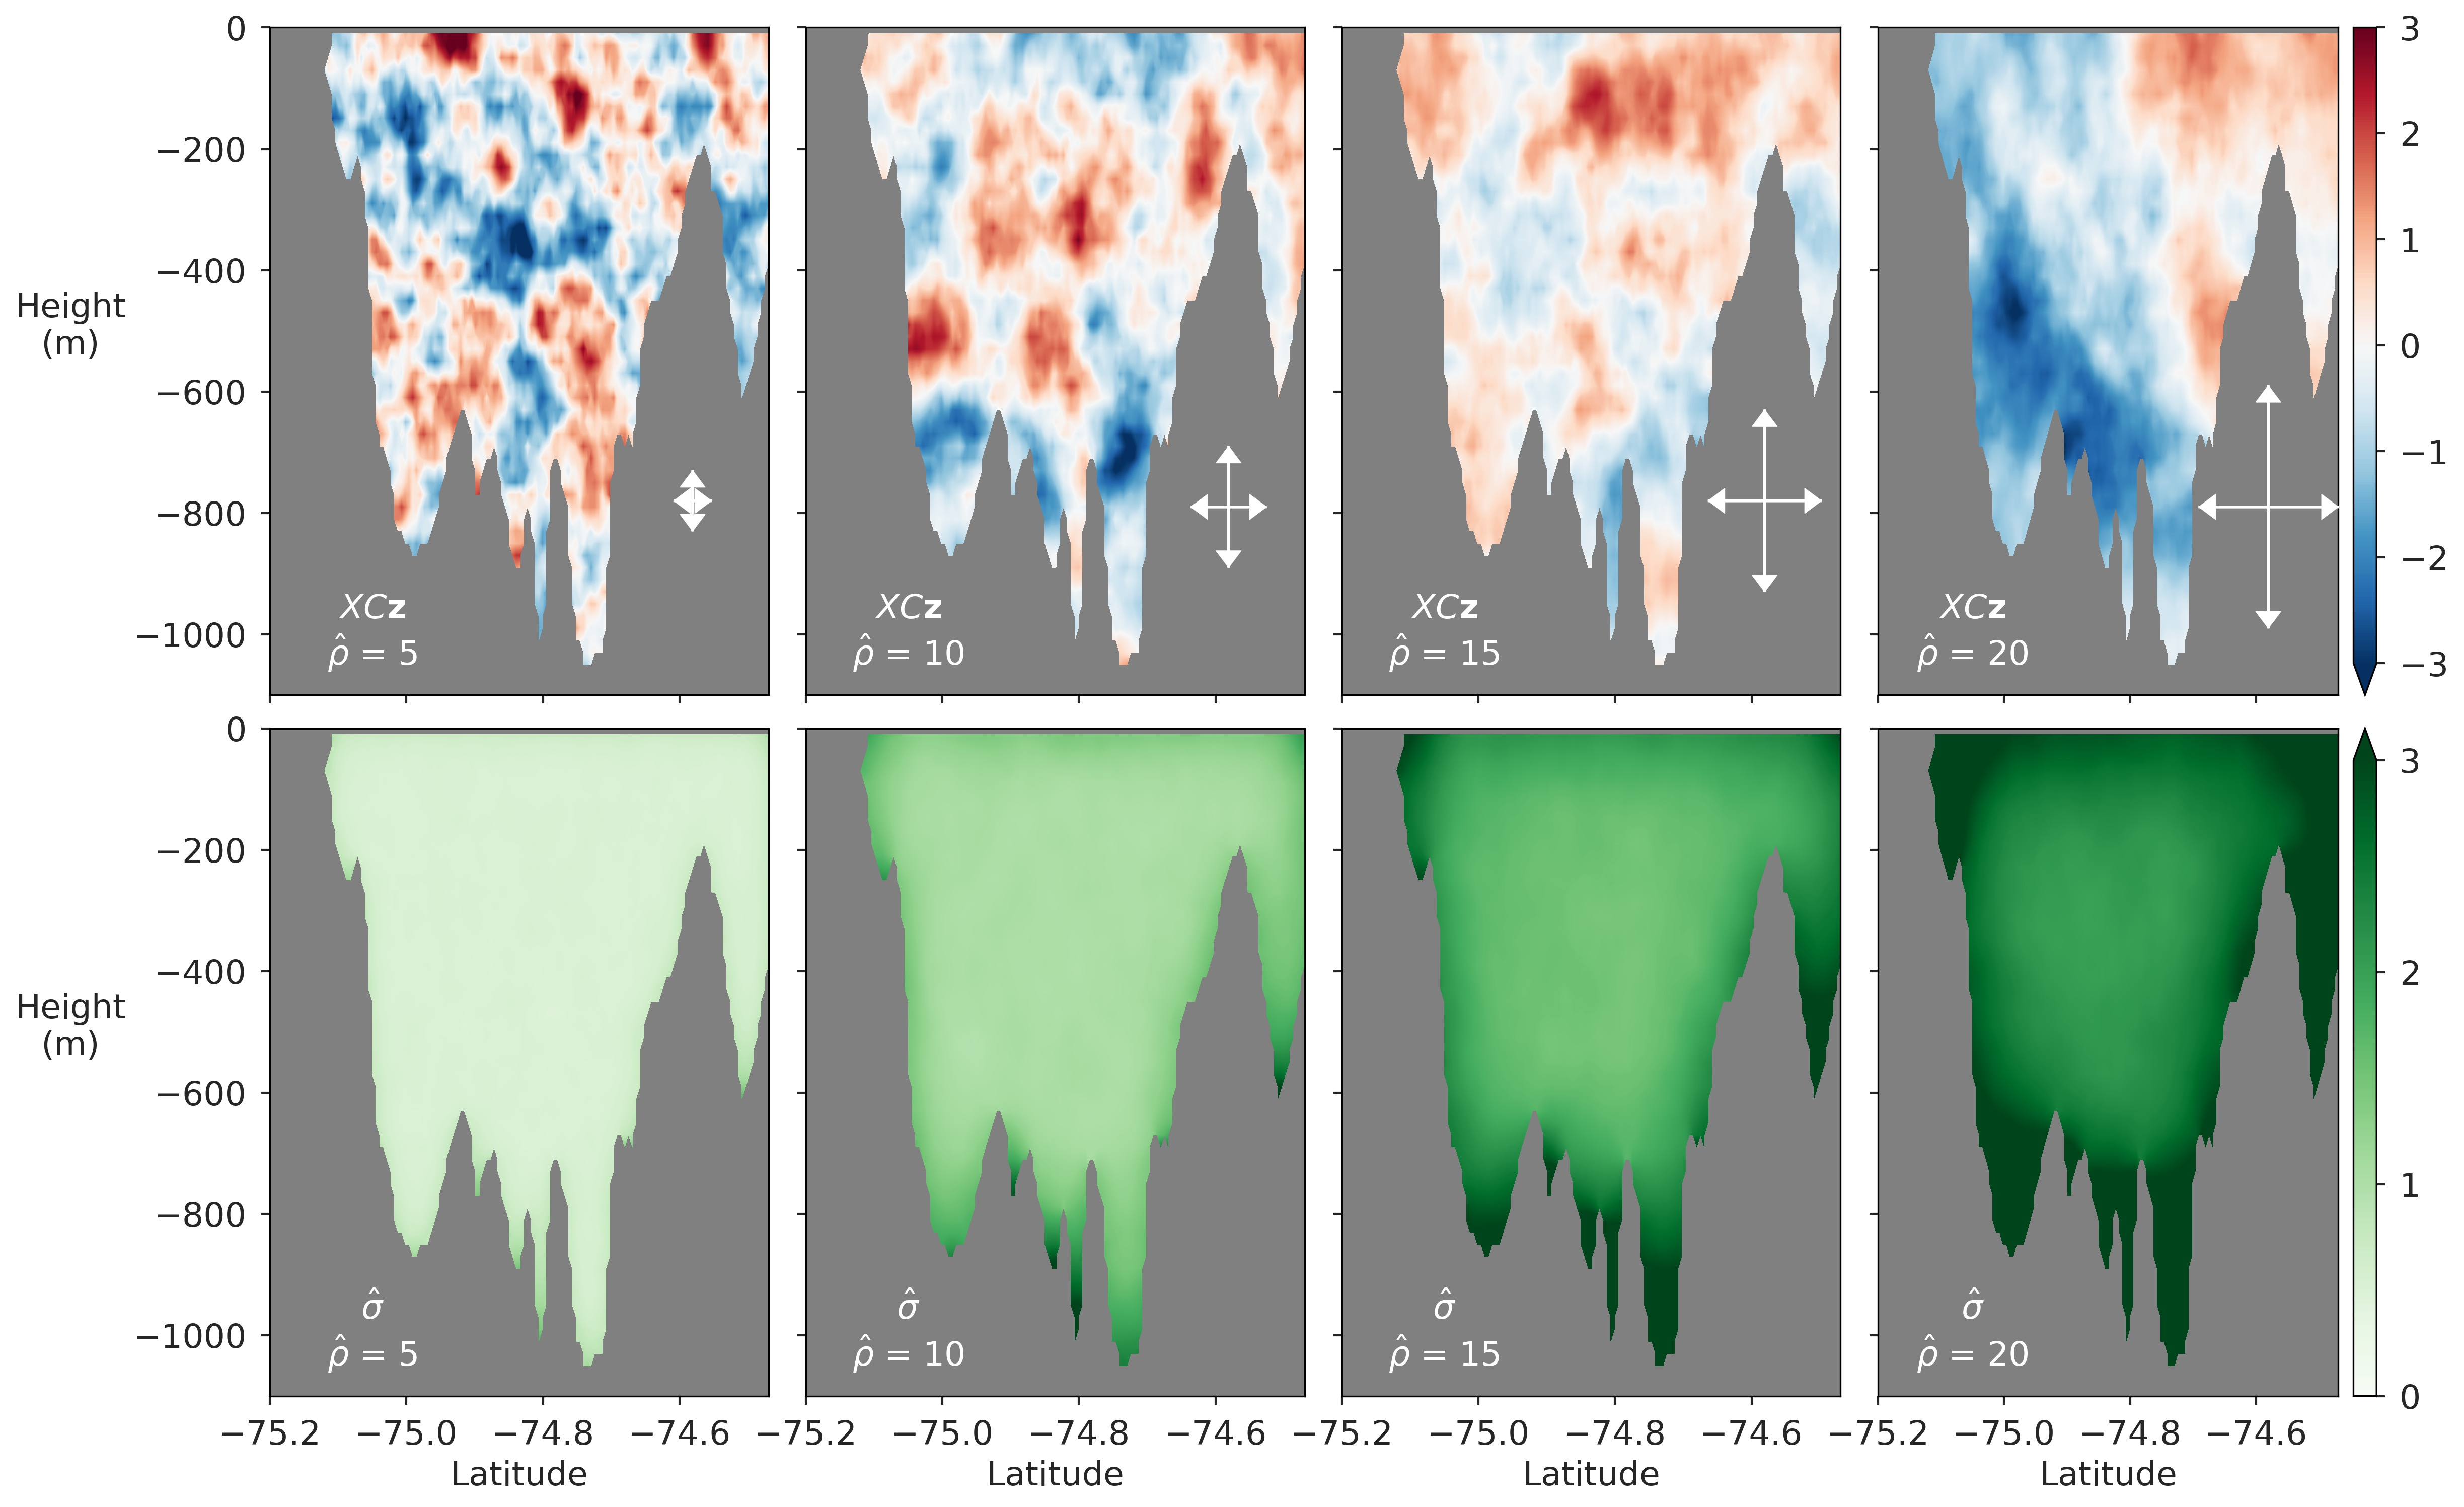
\includegraphics[width=\textwidth]{../figures/samples_and_pointwise_std.jpg}
%    \caption{Normalized samples and pointwise standard deviation from the covariance
%        model.
%        (top row) Samples from the covariance model, normalized by the
%        pointwise standard deviation. Each column shows increasing correlation
%        length scales, which is regulated by $\rangeh$.
%        The arrows in the bottom right corner of each plot show the approximate length scales
%        that are covered by $\rangeh L_y$ and $\rangeh L_z$, respectively.
%        Here we have used $L_y = 2\Delta y_g$ and $L_z=\Delta r_f$, see
%        Figure \ref{fig:mitgcm_grid} for a notational reference.
%        We note that the standard normal vector $\mathbf{z}$ is unique in
%        each figure.
%        (bottom row) Pointwise standard deviation of the covariance operator
%        $CC^T$, estimated from
%        a sample size of $N=1000$. The diagonal matrix $X$ is comprised of the
%        inverse of this field.
%    }
%    \label{fig:matern_samples}
%\end{figure}


\noindent\textbf{Correlation length scales.}

Here we do not use the Jacobian, but just compute based on neighboring grid
cells.
\begin{figure}
    \centering
    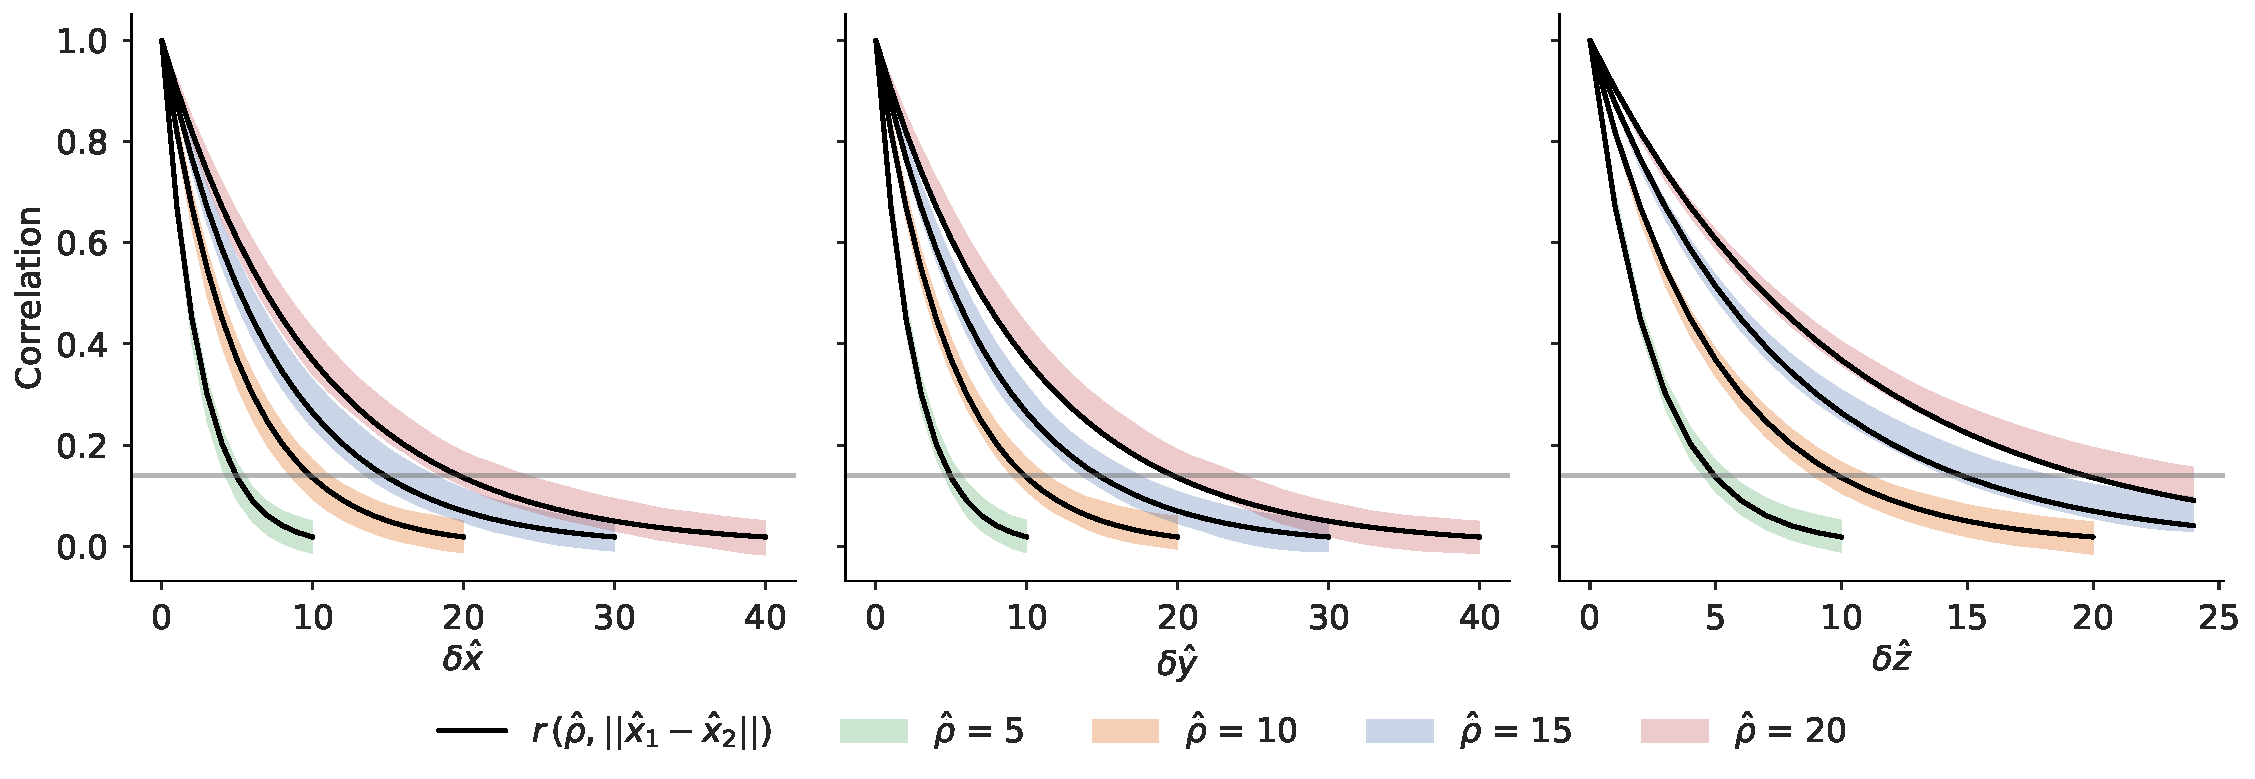
\includegraphics[width=\textwidth]{../figures/matern_llc90_correlation-k25-iy120-ix80-1000samples-4curves.pdf}
    \caption{Correlation coefficient from a subset of the LLC90 in the Pacific
        Ocean, with computations carried out across "inner"
        (158, 118)$^\circ$W,
        (62, 2)$^\circ$S and
        with an "outer" (allowing neighboring interactions spanning out to)
        (178, 98)$^\circ$W,
        (76$^\circ$S, 29$^\circ$N).
        distances computed in each dimension from 1000 samples. The coefficient is
        computed from the random samples used to estimate
        $\hat{\sigma}$ and $X$. Each color denotes correlations computed for a
        different value of $\rangeh$, and the spread is determined by one standard
        deviation around the domain averaged correlation coefficent.
        The black curve denotes the predicted isotropic correlation predicted by
        equation \eqref{eq:matern_correlation_iso} with the appropriate value for
        $\rangeh$.}
    \label{fig:llc90_correlations}
\end{figure}
